%
% LaTeX- Template for Master Theses
%      @ FH Kaernten
%
% V 1.0
% Feb. 2011
% M.Koeberle
%
% Main LaTeX-File
%

\documentclass[a4paper,12pt]{scrreprt}

\usepackage[german,english]{babel}
\usepackage{graphicx}
%\usepackage{lineno}
\usepackage[hang]{caption}
%\usepackage[hang]{subfig}
\usepackage{amsmath}
%\usepackage[light,math]{iwona}
%\usepackage{iwona}
\usepackage{chngcntr} % Zur Nummerierung der Abbildungen in der Reihenfolge 1,2,3...
\counterwithout{figure}{chapter} % Zur Nummerierung der Abbildungen in der Reihenfolge 1,2,3...
\usepackage{hyperref}
\usepackage[utf8x]{inputenc}
\usepackage{fancyhdr}
\usepackage{glossaries}


% ============= Kopf- und Fußzeile =============
\pagestyle{fancy}
%
\lhead{\slshape \leftmark}
\chead{}
\rhead{
\includegraphics[scale=0.15]{pictures/FH_KAERNTEN_logo_rgb_20cm.jpg} 
\includegraphics[scale=0.1]{pictures/Infineon-Logo.svg.png}}
%%
\lfoot{}
\cfoot{\thepage}
\rfoot{}
%%
\renewcommand{\headrulewidth}{0.4pt}
\renewcommand{\footrulewidth}{0pt}

\renewcommand{\baselinestretch}{1.2}
\parindent0em
\parskip1.0ex plus0.5ex minus0.5ex
\voffset-28mm
\hoffset-1in
\topmargin15mm
\headheight5mm
\headsep10mm
\textheight240mm\textwidth160mm
\footskip10mm
\oddsidemargin25mm
\evensidemargin25mm



\def\BS{\textbackslash}
\def\T{\textstyle}

%..........Abkürzungen..........
\makeglossaries
\newacronym{amh}{AMH}{Automated Material Handling}
\newacronym{bpmn}{BPMN}{Business Process Model and Notation}
\newacronym{foup}{FOUP}{Front Opening Unified Pod}
\newacronym{oht}{OHT}{Overhead Hoist Transport}
\newacronym{amhs}{AMHS}{Automated Material Handling System}

%...............................


\begin{document}

\pagestyle{empty}
\pagenumbering{roman}
%
% LaTeX-Template for Master Theses
%	      @ FH Kaernten
%
% V 1.0
% Feb. 2011
% M.Koeberle
%
% Titlepage
%

\thispagestyle{empty}

\selectlanguage{german}
\begin{minipage}[b]{10cm}
Fachhochschule K"arnten \\
Carinthia University of Applied Sciences\\
Integrated Systems and Circuits Design 
\end{minipage}\hfill
\begin{minipage}[b]{5cm}

\includegraphics[height=1.7cm]{./pictures/FH_KAERNTEN_logo_rgb_20cm.jpg}
\end{minipage}
\vspace{1.5cm}
\selectlanguage{english}

\begin{center}
{\huge {\textbf{MASTER THESIS}}}

\vspace{1.5cm}
{\Large {\textbf{ 
\baselineskip25pt
Optimization of tool unloading processes in the semiconductor industry  \\}}}

\vspace{1.5cm}
Submitted in Partial Fulfillment of the Requirements of the Academic Degree\\~\\

Master of Science in Engineering, Msc
\end{center}
\vspace{0.5cm}
\begin{center}
    
\includegraphics[scale=0.25]{pictures/Infineon-Logo.svg.png}
\end{center}

\vspace{0.5cm}
\begin{tabbing}
Registration Number:\hspace{1cm}\= \kill
Author:			\> Thomas Michael Pack, BSc \\~\\
Registration Number:	\> 2110528005 \\~\\
Supervisor:		\> Dipl.-Ing- Dr. techn. Matthias Brandstötter \\
			\> CUAS \\~\\
Company supervisor:	\> Dr. Stefan Schabus  \\
			\> Infineon Technologies Austria AG \\~\\
\end{tabbing}

\vfill
Villach, September 2023


%
% LaTeX-Template for Master Theses
%	 @ FH Kaernten
%
% V 1.0
% Feb. 2011
% M.Koeberle
%
%  Statutory Declaration
%

{\Large \textbf{ Statutory Declaration}}

\vspace{1cm}

I hereby declare that
%
\begin{itemize}
\item 	I have independently written the presented Master thesis by myself.
\item	I have prepared this Master thesis without outside help and without using any sources or aids other than those cited by me; moreover, I have identified as such any passages taken verbatim or in terms of content from the sources used.
\item	in addition, I have fully indicated the use of generative AI models (e.g. ChatGPT) by specifying the product name and the reference source (e.g. URL).
\item   I have not used any other unauthorized aids and have consistently worked independently and when using generative AI models, I realize that I am responsible how the content will be used and to what extent.
\item   I have not yet submitted this Master thesis in the same or similar form to any (other) educational institution as an examination performance or (scientific) thesis.
\item   I am aware that any violation ("use of unauthorized aids") violates academic integrity and may result in (academic-related) legal consequences.
\item	one copy of the Master Thesis is deposited and made available in the CUAS
	library (\textsection 8 Austrian Copyright Law [UrhG]).
\end{itemize} 
%
I fully understand that I am responsible myself for the application for a patent,
trademark or ornamental design and that I have to prosecute any resultant
claims by myself.

\vspace{3cm}

\hrulefill 

(Place, Date) \hfill (Signature)

%
% LaTeX-Template for Master Theses
% 	@ FH Kaernten
%
% V 1.0
% Feb. 2011
% M.Koeberle
%
% Abstract
%

{\Large \textbf{ Abstract}}

\vspace{1cm}



\bigskip
{\textbf{ Key words:}} 
%
% LaTeX-Template for Master Theses
% 	@ FH Kaernten
%
% V 1.0
% Feb. 2011
% M.Koeberle
%
%  Acknowledgement
%

{\Large \textbf{ Acknowledgement}}

\vspace{1cm}



\pagestyle{fancy}
%
% LaTeX-Template for Master Theses
%	 @ FH Kaernten
%
%
% V 1.0
% Feb. 2011
% M.Koeberle
%
% Indices
%

\tableofcontents
\listoffigures
\addcontentsline{toc}{chapter}{List of Figures}
\listoftables
\addcontentsline{toc}{chapter}{List of Tables}

\pagenumbering{arabic}


%
% LaTeX-Template for Master Theses
%	 @ FH Kaernten
%
% V 1.0
% Feb. 2011
% M.Koeberle
%
% Example Chapter 1
%
% Eintieg ins Thema um Grundlagen zu kennen

\chapter{Introduction}





\section{Mobile Industrial Robots}
\label{sec:TopicDescription}

\TeX\ (X or chi is pronounced as in Scottish loch) is a low-level markup and programming language created by Donald Knuth to typeset documents attractively and consistently.
Knuth started writing the \TeX\ typesetting engine in 1977 to explore the potential of the digital printing equipment that was beginning to infiltrate the publishing industry at that time, especially in the hope that he could reverse the trend of deteriorating typographical quality that he saw affecting his own books and articles.
\TeX\ is a programming language, in the sense that it supports the if-else construct, you can make calculations with it (that are performed while compiling the document), etc., but you would find it very hard to make anything else but typesetting with it. The fine control \TeX\ offers makes it very powerful, but also difficult and time-consuming to use. \TeX\ is renowned for being extremely stable, for running on many different kinds of computers, and for being virtually bug free.
Nowadays when producing documents in the \TeX\ language, practically nobody uses plain \TeX. Instead, different \TeX\ distributions such as \LaTeX\ are used to save time, automate certain tasks and reduce user introduced errors.


\section{Unloading Optimization Techniques}
\label{sec:Thoughts}

\LaTeX\ (pronounced either "Lah-tech" or "Lay-tech") is a macro package based on \TeX\ created by Leslie Lamport. Its purpose is to simplify \TeX\ typesetting, especially for documents containing mathematical formulae.
Many later authors have contributed extensions, called packages or styles, to \LaTeX. Some of these are bundled with most \TeX/\LaTeX\ software distributions; more can be found in the Comprehensive \TeX\ Archive Network (CTAN).
Since \LaTeX\ comprises a group of \TeX\ commands, \LaTeX\ document processing is essentially programming. You create a text file in \LaTeX\ markup. The \LaTeX\ macro reads this to produce the final document.
This approach has some disadvantages in comparison with a WYSIWYG (What You See Is What You Get) program such as Openoffice.org Writer or Microsoft Word.

In \LaTeX\:
\begin{itemize}
\item You don't (usually) see the final version of the document when editing it.
\item You generally need to know the necessary commands for \LaTeX\ markup.
\item It can sometimes be difficult to obtain a certain look for the document.
\end{itemize}
On the other hand, there are certain advantages to the \LaTeX\ approach:
\begin{itemize}
\item Document sources can be read with any text editor and understood, unlike the complex binary and XML formats used with WYSIWYG programs.
\item You can concentrate purely on the structure and contents of the document, not get caught up with superficial layout issues.
\item You don't need to manually adjust fonts, text sizes, line heights nor text flow for readability, as \LaTeX\ takes care of them automatically.
\item In \LaTeX\ the document stucture is visible to the user, and can be easily copied to another document. In WYSIWYG applications it is often not obvious how a certain formatting was produced, and it might be impossible to copy it directly for use in another document.
\item The layout, fonts, tables and so on are consistent throughout the document.
\item Mathematical formulae can be easily typeset.
\item Indexes, footnotes, citations and references are generated easily.
\item You are forced to structure your documents correctly.
\end{itemize}
The \LaTeX-like approach can be called WYSIWYM, i.e. What You See Is What You Mean: you can't see what the final version will look like while typing. Instead you see the logical structure of the document. \LaTeX\ takes care of the formatting for you.
The \LaTeX\ document is a plain text file containing the content of the document, with additional markup. When the source file is processed by the macro package, it can produce documents in several formats. \LaTeX\ natively supports DVI and PDF, but by using other software you can easily create PostScript, PNG, JPG, etc.


\section{Problem Description}
\label{sec:ProblemDescription}
In production, time can be lost due to transportation, especially when unloading equipment. As there is currently no specific concept for unloading equipment, transport vehicle congestion can occur. The tools are only unloaded as quickly as possible, but no attention is paid to whether a next batch is already waiting or whether the current one already has a new destination (next process step, storage, etc.). This can result in a subsequent problem, as the lot may have already been stored although it should be sent to the next process and then a new vehicle has to drive to the position to pick it up 
Due to high part variance, the implementation of just-in-time delivery is difficult because the different lots do not have a fixed production sequence. It may be that a lot has to be checked after a process and therefore cannot be transported to the next tool, these checks can usually not be predicted.
For just in time delivery, the materials must arrive exactly when they are needed and are not stored beforehand.
I.e. if a door is delivered in the car industry, it is delivered from the truck directly to the production line and installed.
In the car industry, for example, each individual step has a previous step. One part is gradually added to the whole and it runs along the assembly line. This is also the case in the pharmaceutical industry, where the "ingredients" are gradually added in a certain order to become the finished product.\\


% Problembeschreibung, abstrahiert, Kernproblem, simple Blöcke und Symbole Grafiken mit Worten erklären, Staus, Kreuzungen etc.
% Symbolset
% 
%
% LaTeX-Template for Master Theses
%	 @ FH Kaernten
%
% V 1.0
% Feb. 2011
% M.Koeberle
%
% Example Chapter 2
%

\chapter{Automated Material Handling in Semiconductor Factories}
\label{cha:AMH}



\section{Wafers and Carriers}
\label{sec:WaferCarrier}

A semiconductor factory can have a total building area of around 60.000 m$^2$ which results in a clean room area of roughly 20.000 m$^2$ \cite{InfineonTechnologiesAG.17.07.2023}. In this clean room area the semiconductors are manufactured on substrates, the so called wafers. In Figure \ref{fig:300mmThinWafer} a 300 mm thin wafer which is produced in the new factory of Infineon can be seen.

\begin{figure}[h]
    \centering
    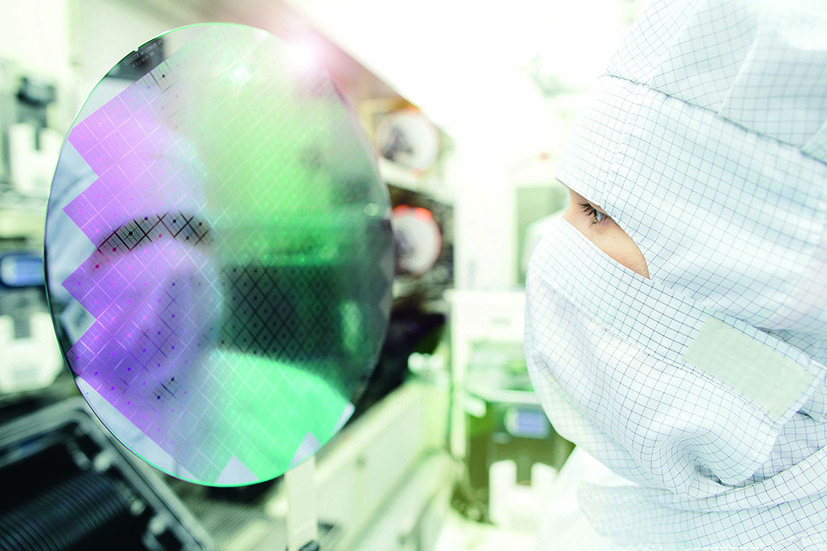
\includegraphics[scale=2.0]{pictures/Infineon-Chipfab-Thin-Wafer-300-mm-Villach.jpg}
    \caption{300 mm Thin Wafer from Infineon \cite{300mmThinWafer.17.09.2021}}
    \label{fig:300mmThinWafer}
\end{figure}

Each wafer starts as a raw and thin disc made out of silicon and is then transformed into integrated circuits. This transformation procedure typically contains between 300 and 700 processing steps that take place on more than 100 manufacturing equipments \cite{monch2012production}. For safer and easier transportation the $\sim$775 μm thick wafers are packed into carriers \cite{Wikipedia.2024}. For the 300 mm wafers the most common type of carrier is the front opening unified pod (\gls{foup}) which can be seen in Figure \ref{fig:Foup}.

\begin{figure}[h]
    \centering
    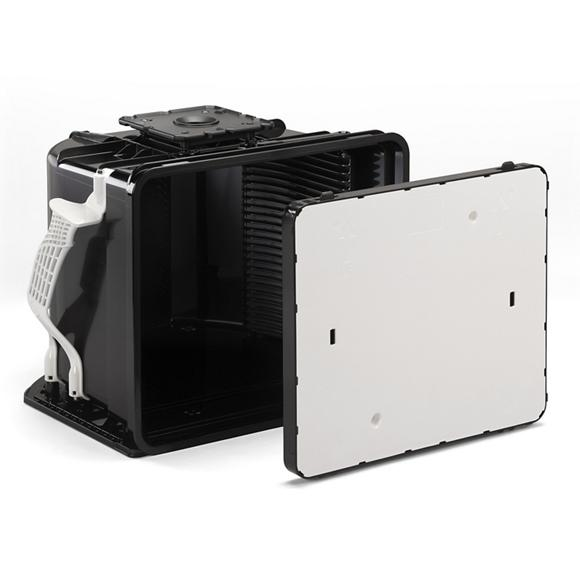
\includegraphics[scale=0.5]{pictures/product-a300g3foupwafercarriers-1-2.jpeg}
    \caption{A300 G3 \gls{foup} Wafer Carrier from Entegris \textbf{Source Needed!!!}} %https://www.entegris.com/shop/en/USD/products/wafer-handling/wafer-processing/300-mm-front-opening-unified-pods-%28foups%29/A300-FOUPs/p/A300FOUPs Quelle hinzufügen
    \label{fig:Foup}
\end{figure}

In a semiconductor plant more than 10,000 carriers are commonly present. One process step has a duration range from a few minutes to 24 hours. The carriers have to be moved between the processes and also the storage. It is important to mention that a \gls{foup} that is waiting to be picked up from the equipment is blocking the loadport of the equipment. On the other hand, an equipment waiting for a new \gls{foup} is not active and therefore does not generate revenue. The transport times between the different manufacturing equipments and storage have to be minimized in order to guarantee high utilization of the equipment. A full \gls{foup} with 25 wafers weighs approximately 9 kg \cite{ManualFoupHandling} and has to be transported between a few meters and more than 200 m. The repeated labour of manual transportation of the \gls{foup}s has been associated with musculoskeletal disorders in human wafer handlers. It is therefore clear that this work should be automated, both from an occupational safety and an economic point of view \cite{ManualFoupHandling}.\newpage

\section{Automated Material Handling (\gls{amh})}
\label{sec:AMH}
Automated Material Handling (\gls{amh}) describes the automated transportation and storage of material in a manufacturing plant. The \gls{foup}s as carriers represent the material that has to be transported in this case. The carriers that are transported or stored in the factory are located in the automated material handling system (\gls{amhs}). The term automated material handling is standardized by the semiconductor equipment and materials international (SEMI) standard through standard documents that are published in the SEMI standard. SEMI is an association of more than 2000 companies world wide active in the electronics design and manufacturing supply chain. Today more than 1000 standards related to electronics are developed and maintained by this association \cite{SEMI}\cite{Semi.org}.


\section{Overhead Hoist Transport (OHT) System}
\label{sec:OHT}


\newpage
\chapter{Business Process Model and Notation}
\label{cha:BPMN}
This chapter focuses on the Business Process Model and Notation (\gls{bpmn}) process modulation standard. First a short overview of the modell will be given. Afterwards the symbols will be described and the advantages of using such a model will be pointed out.\\
Advantage of using \gls{bpmn}

\section{Overview}
\label{sec:BPMNOverview}


Business Process Model and Notation (\gls{bpmn}) is a standard for business process
modeling that provides graphical notation for specifying business processes in a
Business Process Diagram (BPD),2 based on traditional flowcharting techniques.
The objective of \gls{bpmn} is to support business process modeling for both technical
users and business users, by providing notation that is intuitive to business users, yet
able to represent complex process semantics. The \gls{bpmn} 2.0 specification also provides execution semantics as well as mapping between the graphics of the notation
and other execution languages, particularly Business Process Execution Language
(BPEL).3
\gls{bpmn} is designed to be readily understandable by all business stakeholders.
These include the business analysts who create and refine the processes, the technical developers responsible for implementing them, and the business managers who
monitor and manage them. Consequently, \gls{bpmn} serves as a common language,
bridging the communication gap that frequently occurs between business process
design and implementation \cite{Rosing.2015b}.

\section{\gls{bpmn} Symbols}
\label{sec:BPMNSymbols}

\section{Advantage of using \gls{bpmn}}
\label{sec:BPMNGoal}
\chapter{Modeling}
\label{cha:Modeling}

% Eventuell Modeling und Simulation zusammenführen wenn beide eigenständig zu wenig Seiten haben
% Berechnungen, aus dem BPMN Modell
% Investieren in die Analyse des Models,
% Denkbar, abgespeckte variante der Simulation durchzuführen, entweder freie software oder selbstprogrammiert
% Wenn selbst schreiben dann brauche ich die Basisformularitäten, Kombination aus modulen/atomare Einheiten, diese beschreiben, Schnittstellen beschreiben, was passiert wenn ich von einer atomaren Einheit zur nächste übergehe
% Systemzustand möchten wir berechnen, gibt alle informationen preis in denen sich das System gerade befindet
% Zustand dann beschreiben mit bestimmten Regelwerken, wenn mehrere Buffer hintereinander stehen werden sie am Anfang vermutlich leer stehen, ab welchem Zeitpunkt ist Buffer immer leer -> das wäre der Anfang
% Komplexere Fragestellungen immer komplexer



\section{1}
\label{sec:}
\chapter{AMHS and OHT Simulation Environment}
\label{cha:SimEnvironment}

\section{Software Components}
\label{sec:SWComponents}

\section{Simulation Parameters}
\label{sec:SimParameters}

\section{Validation of Simulation}
\label{sec:SimValidation}
\chapter{Evaluation of Results and Behaviour Analysis}
\label{cha:Eval}

\section{Unloading Strategy A}
\label{sec:MethodA}


\section{Unloading Strategy B}
\label{sec:MethodB}

\section{Unloading Strategy C}
\label{sec:MethodC}
\chapter{Conclusion and Outlook}
\label{cha:Conclusion}

\section{Summary}
\label{sec:summary}

\section{Further Optimization }
\label{sec:Further}

\section{Conclusion and Outlook}
\label{sec:Recommendation}


\addcontentsline{toc}{chapter}{Bibliography}
\bibliographystyle{unsrtdin}
\bibliography{bib}
\printglossaries
%%
% LaTeX-Template for Master Theses
% 	@ FH Kaernten
%
% V 1.0
% Feb. 2011
% M.Koeberle
%
% List of Abbreviations
%

\chapter*{List of Abbreviations}
\addcontentsline{toc}{chapter}{List of Abbreviations}

\begin{tabular}{ll}
AMH		& Automated Material Handling \\
BPMN    & Business Process Model and Notation \\
FOUP    & Front Opening Unified Pod\\
OHT		& Overhead Hoist Transport \\

BSIM		& Berkeley Short-channel IGFET Model \\ 
		& refers to a family of MOSFET transistor models for integrated circuit design \\
VHDL		& \textbf {V}ery High Speed Integrated Circuit \textbf {H}ardware \textbf {D}escription \textbf {L}anguage

\end{tabular}

%%
% LaTeX-Template for Master Theses
% 	@ FH Kaernten
%
% V 1.1
% (c) Thomas Klinger / Dezember 1998
% überarbeitet im Oktober 1999
%
% V 1.2	
% modified for master theses
% Feb. 2011
% M.Koeberle
%
% Appendix
%

\appendix
\addcontentsline{toc}{chapter}{Appendix}

\chapter{Source Code}
\section{Template File Formats}
\subsection{HSPICE}

\label{table:template_cdl}
{\footnotesize
\begin{verbatim}
HEADER_FIRST: .SUBCIRCUIT &!cell_name &%I &%O &%IO &%S &@BulkNode 
PIN_INFO: *.PININFO &( &%I : I &) \&( &%O : O &) &( &%IO : IO &) 
STOP_VIEW: M &^ &!inst_name &@d &@g &@s &@BulkNode nmos w= &@w l= &@l 
INSTANCE: X &^ &!inst_name &%I &%O &%IO &!cell_name
\end{verbatim}
}

\subsection{VHDL}

\label{table:template_vhdl}
{\footnotesize
\begin{verbatim}
HEADER_FIRST ENTITY &!cell_name IS \n
    \t PORT( \n  \t &( &%I : IN std_logic; \n
    &)  \t &( &%O : OUT std_logic; \n
    &) ); END &!cell_name NULL

PIN_INFO \n ARCHITECTURE madebyTDI of &!cell_name IS \n
    \t &( SIGNAL &( &%I : std_logic; \n
    &)  \t &( &%O : std_logic; \n
    &) BEGIN NULL

INSTANCE \t X &- &!inst_name : &!cell_name \n
    \t PORT MAP( \n
    \t  \t  &( IN => &%I , \n
    &) \t   \t  &( OUT => &%O , \n
    &) );  NULL

FOOTER END madebyTDI; NULL
\end{verbatim}
}

\section{Generated Netlists}

\subsection{HSPICE}
\label{table:net_hspice}

{\footnotesize
\begin{verbatim}
**  Cell 'c_inv', library: 'cmoslib', path
** '/opt/tech5/cmos/.dr/cmoslib/v2.1/cdb/cmoslib', vers 'vnil'
.SUBCKT c_inv in0 out0 hSup lSup nBulk pBulk n0L=1.0 n0W=1.0 p0L=1.0 p0W=1.0
*.PININFO in0:I out0:O

** The following net names were mapped:
** OriginalName: net11 mapped to: hSup
** OriginalName: net10 mapped to: lSup

Mn0 out0 in0 lSup nBulk nmod  w='n0W*GEONSHRNK-2*GEONDEL2'
+ l='n0L*GEONSHRNK-2*GEONDEL1'
Mp0 out0 in0 hSup pBulk pmod  w='p0W*GEOPSHRNK-2*GEOPDEL2'
+ l='p0L*GEOPSHRNK-2*GEOPDEL1'

.ENDS

**  Cell 'roli_einfach', library: 'rol', path
** '/home/sab_kurs/fw1.1.1/v1.0.0/home/leng/lib_rol/rol', vers 'vnil'
XIN0 input output VDD VSS VSS VDD c_inv n0L=n0L p0L=p0L n0W=n0W p0W=p0W
\end{verbatim}
}

\subsection{VHDL}
\label{table:net_vhdl}
{\footnotesize
\begin{verbatim}
--Netlist:
--Time: Tue Jan 11 11:41:47 2000
--By: leng

--Library=cmoslib,Cell=c_inv,View=native
LIBRARY IEEE,cmoslib,proj_vhdl,proj_verilog;
USE IEEE.std_logic_1164.all;
USE work.all;
USE cmoslib.cmoslib.all;

ENTITY c_inv IS
     GENERIC (
          n0L : real := 1.0;
          n0W : real := 1.0;
          p0L : real := 1.0;
          p0W : real := 1.0
     );
     PORT(
          in0 : IN std_logic;
          out0 : OUT std_logic
     );
END c_inv;

ARCHITECTURE madebyTDI OF c_inv IS
     SIGNAL VSS : std_logic;
     SIGNAL VDD : std_logic;

     SIGNAL out0_ylw : std_logic;

BEGIN

     VSS <= '0';
     VDD <= '1';
     out0 <= out0_ylw;
     Mn0 : c_ntrans
          PORT MAP(
               d => out0_ylw,
               s => VSS,
               g => in0
          );

     Mp0 : c_ptrans
          PORT MAP(
               d => out0_ylw,
               s => VDD,
               g => in0
          );

END madebyTDI;
\end{verbatim}
}


\end{document}
